\documentclass[fontsize=13pt,a4paper,DIV=15,parskip=half]{scrartcl}

\usepackage[utf8]{inputenc}
\usepackage[dvipsnames]{xcolor}
\usepackage[hyperindex]{hyperref}
\usepackage{lastpage}
\usepackage{tikz}
\usepackage{tikzpagenodes}
\usepackage{pgfplots}
\usepackage{enumitem}
\usepackage{scrlayer-scrpage}
\usepackage{xspace}
\usepackage{float}
\usepackage{amsfonts,amsmath,amsthm}
\usepackage{thmtools}
\usepackage[english]{babel}
\usepackage[autostyle, style=english]{csquotes}
\usepackage{wrapfig}
\usepackage{subcaption}
\usepackage{listings}
\usepackage[backend=biber,style=alphabetic]{biblatex}
\addbibresource{bib.bib}
\usepackage{mleftright}
%\usepackage{BOONDOX-calo}
%\usepackage{dsfont}
\usepackage{tikz-cd}
\usepackage[framemethod=TikZ]{mdframed}
\usepackage{soulutf8}
\usepackage{mathtools}
\usepackage{multicol}
\usepackage{nameref}
\usepackage{stmaryrd}
\usepackage{fvextra}
\usepackage{adjustbox}
\usepackage{fontawesome}
\usepackage{fontspec}
\usepackage{mathpartir}
\usepackage{etoolbox}
\usepackage{todonotes}
\usepackage{verbatim}
\usepackage{algorithm}
\usepackage[rightComments=false,beginComment=$\qquad\triangleright$~]{algpseudocodex}
\usepackage{ebproof}
\usepackage[makeroom, thicklines]{cancel}
\renewcommand{\CancelColor}{\color{nicered}}
\usepackage{setspace}
\usepackage{fourier-otf}
\setmathfont{Erewhon-Math.otf}[CharacterVariant={20}]
%\usepackage{pxfonts}
%\usepackage[scaled=0.92]{mathpazo}
\usepackage{juliamono}
\usepackage[osf]{Alegreya}
\usepackage[osf]{AlegreyaSans}
\let\mathds\mathbb
%\DeclareMathAlphabet{\mathsf}{OT1}{cmss}{m}{n}

\renewcommand{\mathsf}[1]{\text{\normalfont\sffamily#1}}
\renewcommand{\texttt}[1]{\text{\normalfont\ttfamily#1}}

\ebproofset{right label template=$\inserttext$, left label template=\tiny$\inserttext$, center=false}

\RedeclareSectionCommand[beforeskip=0.10em, afterskip=0.10em]{section}
\RedeclareSectionCommand[beforeskip=0.05em, afterskip=0.001em plus 0em]{subsection}


\fvset{bgcolor=lightgray!10,backgroundcolorpadding=3pt}

\MakeOuterQuote{"}

\newcommand\redQuestionBox{
  \tikz[baseline]{
    \node[rectangle,fill=nicered,anchor=base,rounded corners=2pt] (A) {\color{white}\textsf{\textbf{?}}\ensuremath{\,}};
  }
}

\colorlet{deeppurple}{DarkOrchid}
\colorlet{deepgreen}{ForestGreen!70!black}
\colorlet{deepblue}{NavyBlue!70!black}
\colorlet{deepred}{RawSienna!70!black}
\colorlet{nicered}{BrickRed!70!white}

\makeatletter
\g@addto@macro\bfseries{\boldmath}
\makeatother

\lstset{
  basicstyle=\small\ttfamily,
  captionpos=b,
  escapeinside={@}{@},
  mathescape=true,
  language=sql,
  frame=leftline,
  framesep=1em,
  backgroundcolor=\color{gray!10},
  morekeywords={with, over, rank, partition}
}

\hypersetup{
  colorlinks,
  citecolor=deepgreen,
  filecolor=nicered,
  linkcolor=deepblue,
  pdfencoding=auto,
  psdextra,
  urlcolor=deepred
}

\usetikzlibrary{positioning,shadings,arrows.meta,fit}

\clearpairofpagestyles

\newcommand\showpage{\itshape\hfill--~\thepage/\pageref*{LastPage}~--\hfill}
\cofoot[\showpage]{\showpage} \cefoot[\showpage]{\showpage}

\setlist[enumerate]{font={\bfseries\color{deepblue}}}
\AtBeginDocument{
  \renewcommand{\labelitemi}{\bfseries\color{deepblue}$\triangleright$}
  \renewcommand{\labelitemii}{\bfseries\color{deepblue}–}
  \renewcommand{\labelitemiii}{\bfseries\color{deepblue}•}
}

\newcommand\separatorBlock{
  \raisebox{-0.2em}{
    \tikz{ \draw[deepblue,ultra thick, line cap=round] (0,0) -- (0,1em); }
  }
}

\newcommand\vertical[1]{
  \rotatebox[origin=c]{270}{\ensuremath{#1}}
}

\mdfsetup{skipabove=1em,skipbelow=0em,linewidth=0pt,rightline=false, topline=false, bottomline=false}


\theoremstyle{definition}

\declaretheoremstyle[
  headfont=\bfseries\sffamily\color{deepgreen}, bodyfont=\normalfont,
% mdframed={
%   linecolor=ForestGreen, % backgroundcolor=ForestGreen!5,
% },
]{thmgreenbox}

\declaretheoremstyle[
  headfont=\bfseries\sffamily\color{deepblue}, bodyfont=\normalfont\sffamily\itshape,
% mdframed={
%   linecolor=NavyBlue,% backgroundcolor=NavyBlue!5,
% },
]{thmbluebox}

\declaretheoremstyle[
  headfont=\bfseries\sffamily\color{deepblue}, bodyfont=\normalfont,
  mdframed={
    linecolor=deepblue,
    linewidth=2pt,
  },
  numbered=no,
]{thmblueline}

\declaretheoremstyle[
  headfont=\bfseries\sffamily\color{deepred}, bodyfont=\normalfont,
% mdframed={
%   linecolor=RawSienna,% backgroundcolor=RawSienna!5,
% },
]{thmredbox}

\declaretheoremstyle[
  headfont=\itshape\sffamily\color{deepred}, bodyfont=\normalfont,
% mdframed={
%   linecolor=RawSienna,% backgroundcolor=RawSienna!1,
%   linewidth=0pt,
% },
  numbered=no,
  qed=\qedsymbol,
]{thmproofbox}

\newcommand\defineMarkerColor[2]{
  \AtBeginEnvironment{#1}{
    \setlist[enumerate]{font={\color{#2}}}
    \renewcommand{\labelitemi}{\color{#2}\small$\triangleright$}
    \renewcommand{\labelitemii}{\color{#2}–}
    \renewcommand{\labelitemiii}{\color{#2}•}
    \renewcommand\emph[1]{{\bfseries\em\color{#2}##1}}
  }
}


\AtBeginDocument{
  \setlist[enumerate]{font={\bfseries\color{deepblue}}}
  \renewcommand{\labelitemi}{\bfseries\color{deepblue}\small$\triangleright$}
  \renewcommand{\labelitemii}{\bfseries\color{deepblue}–}
  \renewcommand{\labelitemiii}{\bfseries\color{deepblue}•}
}


\setlist[enumerate]{font={\color{deepblue}}}
\renewcommand{\labelitemi}{\color{deepblue}\small$\triangleright$}
\renewcommand{\labelitemii}{\color{deepblue}–}
\renewcommand{\labelitemiii}{\color{deepblue}•}

\declaretheorem[style=thmgreenbox, name=Axiom, numbered=no]{axi} \defineMarkerColor{axi}{deepgreen}
\declaretheorem[style=thmgreenbox, name=Definition]{defn} \defineMarkerColor{defn}{deepgreen}
\declaretheorem[style=thmbluebox, name=Example]{exm}      \defineMarkerColor{exm}{deepblue}
\declaretheorem[style=thmbluebox, name=Exercise]{exo}     \defineMarkerColor{exo}{deepblue}
\declaretheorem[style=thmbluebox, name=Question, parent=section]{que}     \defineMarkerColor{que}{deepblue}
\declaretheorem[style=thmredbox, name=Proposition]{prop}  \defineMarkerColor{prop}{deepred}
\declaretheorem[style=thmredbox, name=Theorem]{thm}      \defineMarkerColor{thm}{deepred}
\declaretheorem[style=thmredbox, name=Lemma]{lem}         \defineMarkerColor{lem}{deepred}
\declaretheorem[style=thmredbox, name=Corollary]{crlr}   \defineMarkerColor{crlr}{deepred}
\declaretheorem[style=thmblueline, name=Remark]{rmk}    \defineMarkerColor{rmk}{deepblue}
\declaretheorem[style=thmblueline, name=Note]{note}       \defineMarkerColor{note}{deepblue}
\declaretheorem[style=thmproofbox, name=Proof]{replacementproof}
\newenvironment{prv}[1][\proofname]{\vspace{-12pt}%
\begin{replacementproof}}{\end{replacementproof}} \defineMarkerColor{prv}{deepred}
\declaretheorem[style=thmproofbox, name=Proof idea]{replacementideaproof}
\newenvironment{prvid}[1][\proofname]{\vspace{-12pt}%
\begin{replacementideaproof}}{\end{replacementideaproof}} \defineMarkerColor{prvid}{deepred}

\RequirePackage{caption}
\DeclareCaptionLabelFormat{labelformat}{\textbf{#1~#2}\separatorBlock}
\captionsetup{labelformat=labelformat,labelsep=none,textfont=sl}

\DeclareMathSizes{11}{9}{7}{5}

\title{Computational Geometry and Digital Images -- \textit{Project Report}}
\author{Hugo \textsc{Salou}}

\let\emph\relax
\DeclareTextFontCommand{\emph}{\bfseries\em\color{deepblue}}

\renewcommand{\thefootnote}{\alph{footnote}}

\tikzcdset{arrow style=math font}
\tikzset{
  equiv/.style={-,preaction={draw,double equal sign distance}},
  >=Straight Barb,
}

\newcommand\linkfile[1]{\href{https://gitlab.aliens-lyon.fr/hsalou/m1-cgdi-project/-/blob/master/#1}{\texttt{#1}}}

\begin{document}
  \begin{center}
    \bfseries
    \sffamily

    {\large\itshape ---\hspace{1em}Project Report\hspace{1em}---}

    {\huge Computational Geometry}

    \vspace{-0.75em}

    {\LARGE\textit{and}}

    \vspace{-0.5em}

    {\huge Digital Images}

    {\large \itshape Hugo SALOU}
  \end{center}

  \section{Context of this project.}

  Three dimensional meshes are based on a finite set of triangles. The smaller
  this set, the faster we are able to do operate on that 3D object (applying
  some transformation on the vertices, displaying it, doing physical
  simulations, \textit{etc}). It is thus crucial to keep a low number of
  triangles in, for example, real-time applications. Lowering the number of
  triangles also allows for a lower memory footprint for assets. This idea is
  closely related to \textit{procedural generation} of 3D models, textures,
  \textit{etc}: trading "ahead-of-time" generation for "run-time" generation.
  This generation at run-time is more costly that simply reading pre-computed
  results from a file. However, in some cases, the run-time computation can be
  done in parallel, on the GPU.

  \section{Presentation of curved PN triangles \cite{curvedpntriangles}.}

  This project is based on~\cite{curvedpntriangles}. They provide an algorithm
  to take a 3D mesh with a small number of triangles, and turn in into a finer,
  more detailed mesh. This initial mesh must contain normal vectors on each
  vertex, instead of each triangle. This is called a \textit{point-normal (PN)
  triangle mesh}.

  Each PN triangle is then \textit{curved} (hence the name of the paper) in
  coherence with the direction of the normal vectors at the triangle's
  vertices. This "curving" is done using a cubic Bézier patch
  (figure~\ref{fig:process}, page~\pageref{fig:process}).

  \begin{figure}[h]
    \centering
    \subcaptionbox{Initial PN triangle}{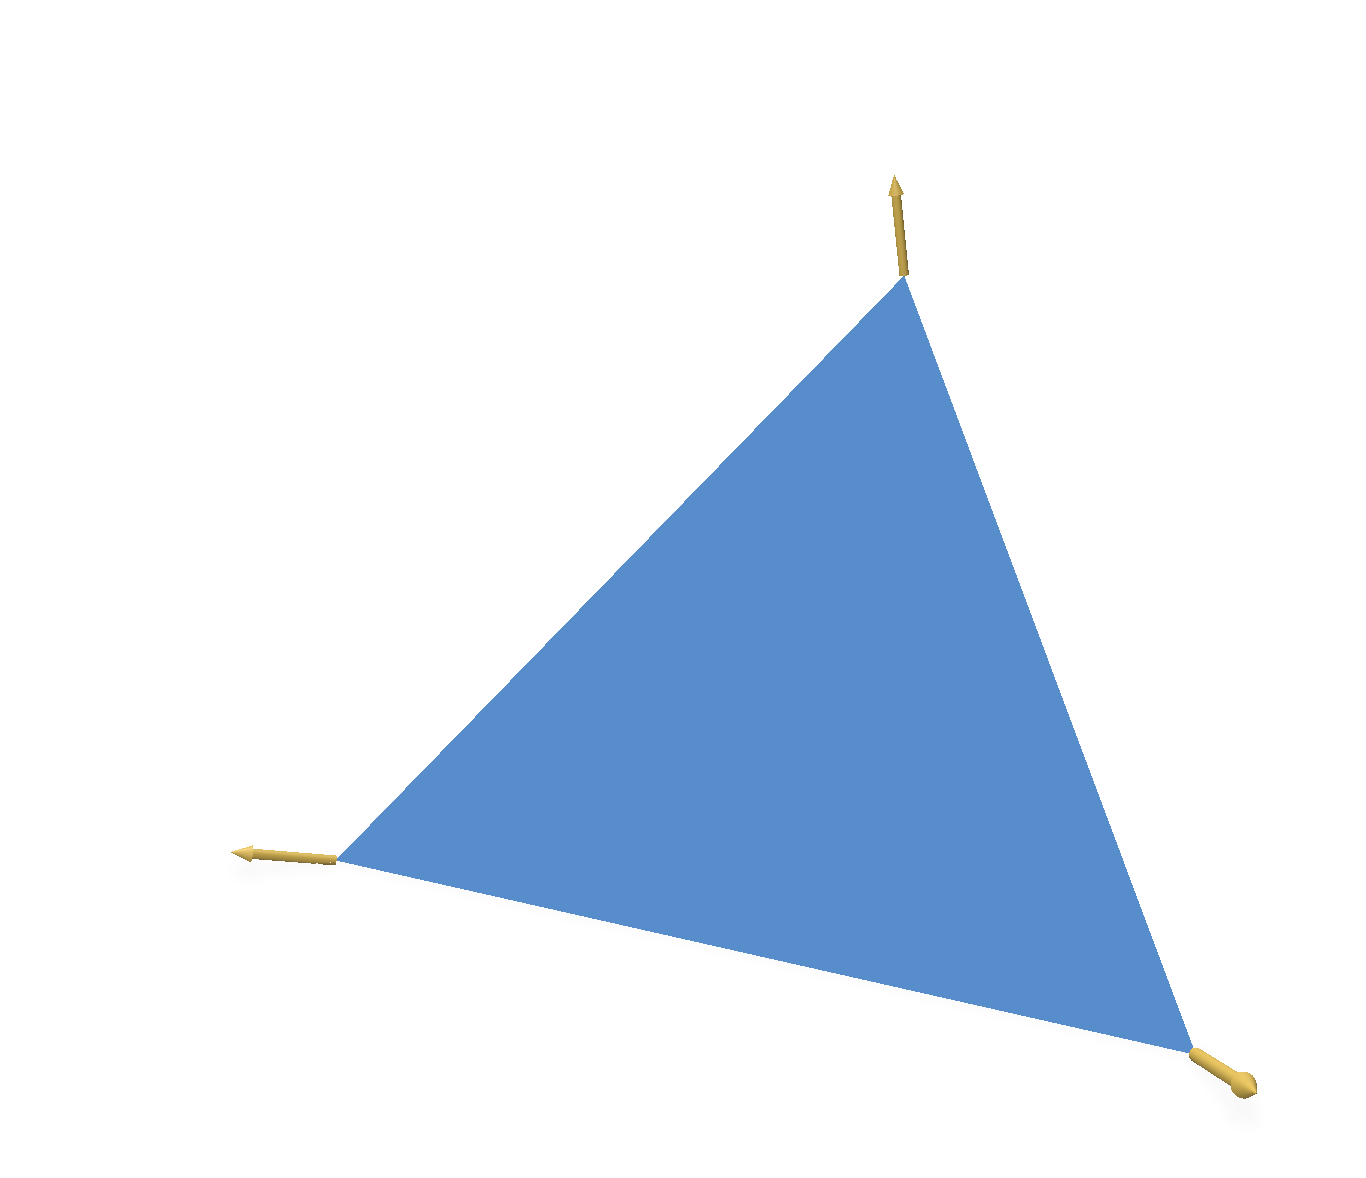
\includegraphics[width=0.32\textwidth]{figures/start.png}}
    \subcaptionbox{Generated Bézier patch}{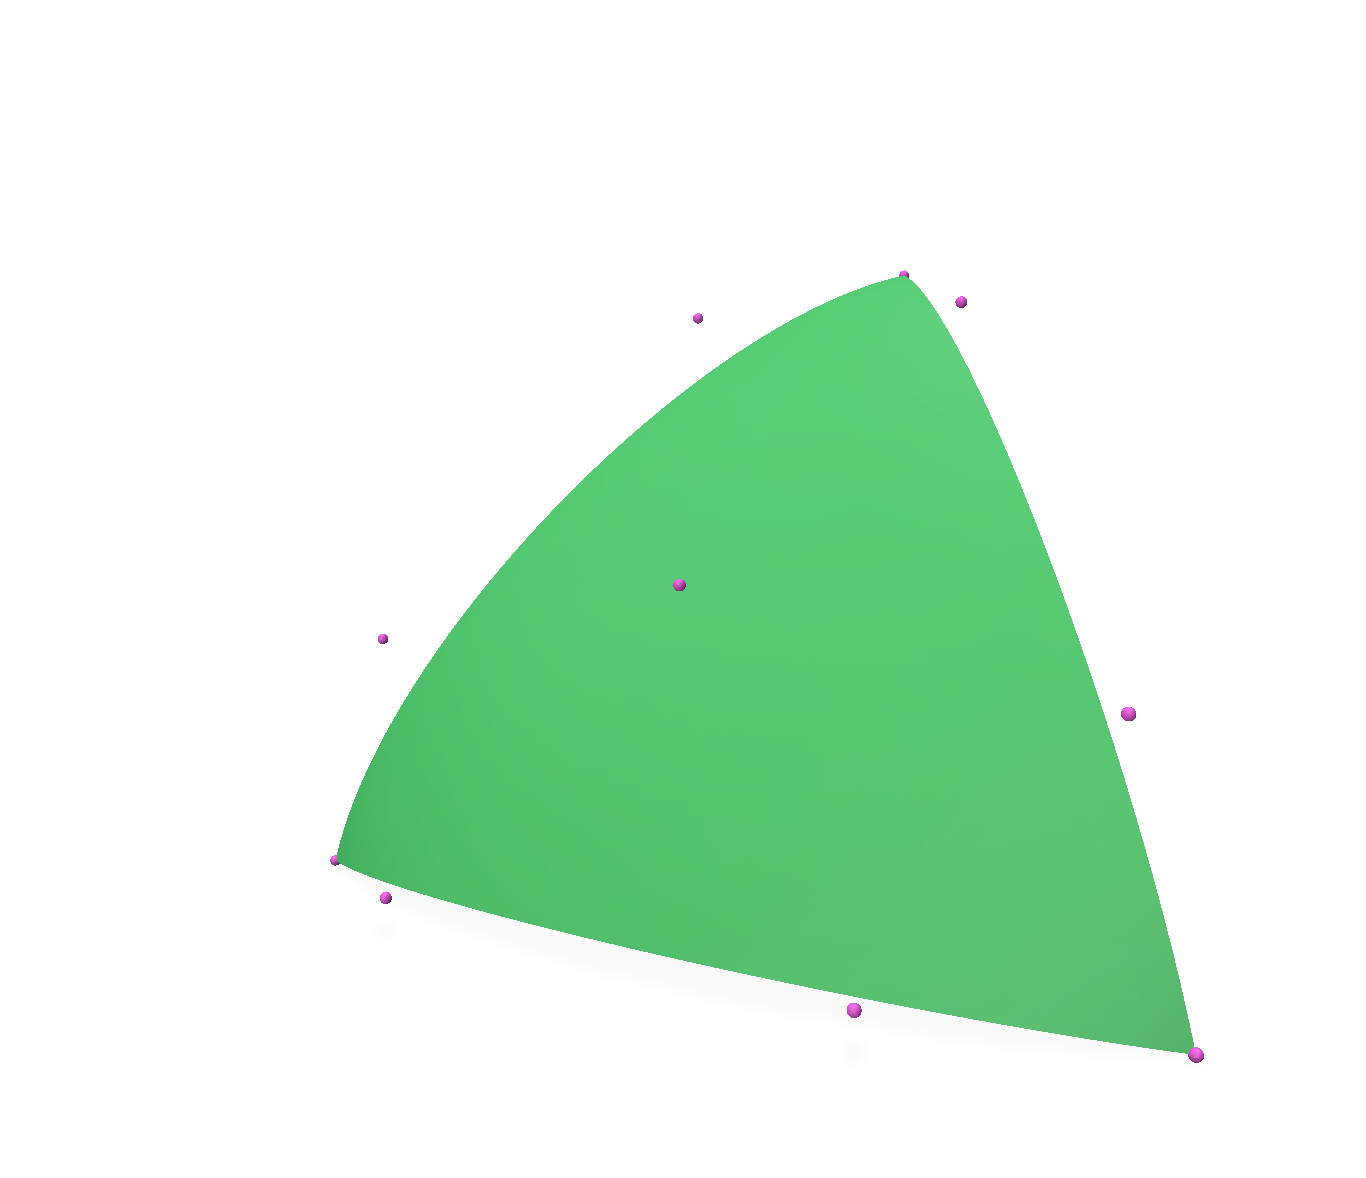
\includegraphics[width=0.32\textwidth]{figures/curved.png}}
    \subcaptionbox{Side view of the patch}{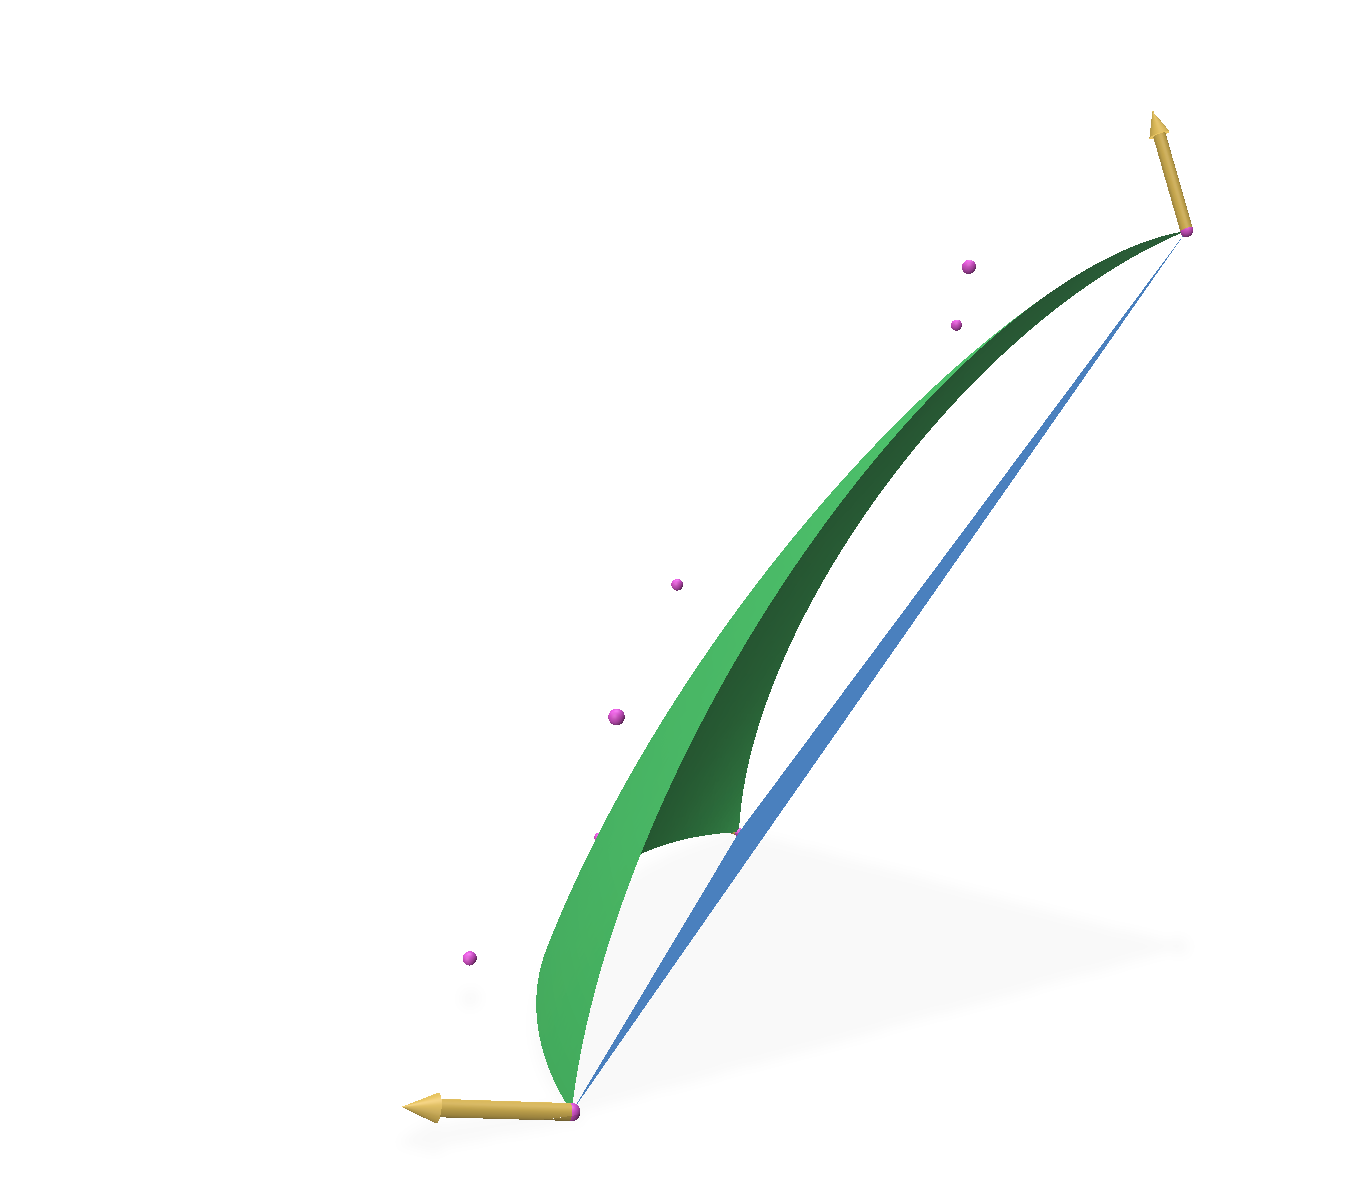
\includegraphics[width=0.32\textwidth]{figures/side.png}}
    \caption{A PN triangle and its associated curved PN triangle.}
    \label{fig:process}
  \end{figure}

  A Bézier patch is given as the following parametric surface
  \[
  \begin{array}{rrcl}
    \vec b:& \Delta &\longrightarrow &\mathds{R}^3 \\
           &(u,v, w)&\longmapsto& \sum_{i+j+k=3} \vec b_{kij} \: u^i v^j w^k
  ,\end{array}
  \quad \text{ where }  \quad
  \Delta := \mleft\{\,(u, v,w) \;\middle|\;
    \begin{array}{l}
      u,v,w \ge 0\\
      u + v + w = 1
    \end{array}
  \,\mright\}.
  \]

  Given a PN triangle whose vertices' positions are $\vec P_1, \vec P_2, \vec
  P_3$ and vertices' normals are $\vec N_1, \vec N_2, \vec N_3$, we define the values of
  control points $\vec b_{kij}$ (shown in magenta in figure~\ref{fig:process})
  as follow
  \begin{align*}
    \vec{b}_{300} &:= \vec{P}_1, & 
    \vec{b}_{030} &:= \vec{P}_2, & 
    \vec{b}_{003} &:= \vec{P}_3,
  \end{align*}
  \vspace{-2\baselineskip}
  \begin{align*}
    \vec{b}_{012} &= \frac{1}{3} ( 2 \vec{P}_{3} + \vec{P}_{2} - w_{32}\vec{N}_{3}), &
    \vec{b}_{021} &= \frac{1}{3} ( 2 \vec{P}_{2} + \vec{P}_{3} - w_{23}\vec{N}_{2}), &&\\
    \vec{b}_{102} &= \frac{1}{3} ( 2 \vec{P}_{3} + \vec{P}_{1} - w_{31}\vec{N}_{3}), &
    \vec{b}_{201} &= \frac{1}{3} ( 2 \vec{P}_{1} + \vec{P}_{3} - w_{13}\vec{N}_{1}), &&\\
    \vec{b}_{120} &= \frac{1}{3} ( 2 \vec{P}_{2} + \vec{P}_{1} - w_{21}\vec{N}_{2}), &
    \vec{b}_{210} &= \frac{1}{3} ( 2 \vec{P}_{1} + \vec{P}_{2} - w_{12}\vec{N}_{1}), &
  \end{align*}
  \vspace{-2\baselineskip}
  \begin{align*}
    \vec{b}_{111} := \alpha \vec{E} + (1 - \alpha) \vec{V}
  ,\end{align*}
  where
  \begin{itemize}
    \item $w_{ij} := ( \vec{P}_{j} - \vec{P}_{i} ) \cdot \vec{N}_{i}$,
    \item $\vec{E} := \frac{1}{6} (\vec{b}_{012} + \vec{b}_{021} + \vec{b}_{102} + \vec{b}_{201} + \vec{b}_{120} + \vec{b}_{210})$,
    \item $\vec{V} := \frac{1}{3} (\vec{P}_{1} + \vec{P}_{2}+ \vec{P}_{3})$.
  \end{itemize}

  \begin{wrapfigure}[8]{r}{0.3\textwidth}
    \vspace{-2cm}
    \centering
    
\includegraphics[width=0.35\textwidth]{figures/alpha.png}
    \vspace{-1.5cm}
    \caption{Influence of $\alpha$.}
    \label{fig:alpha}
  \end{wrapfigure}

  Changing the value of $\alpha$ changes how "bumpy" the triangle gets
  (figure~\ref{fig:alpha}). In \cite{curvedpntriangles}, the value of $\alpha$
  is set to $1/2$. 
  Figure~\ref{fig:alpha} shows curved PN triangles obtained with different
  values for $\alpha$ (sliced view in the middle of triangle). In
  figure~\ref{fig:alpha}, the "most bumpy" (outwards) PN triangle, in yellow,
  corresponds to $\alpha = 2$. Other values are, in order, \[
  \alpha = 1.5, \quad 1.0, \quad 0.75, \quad 0.5, \quad 0.25, \quad 0.0
  .\]
  \begin{wrapfigure}[7]{l}{0.35\textwidth}
    \centering
    \vspace{-1cm}
    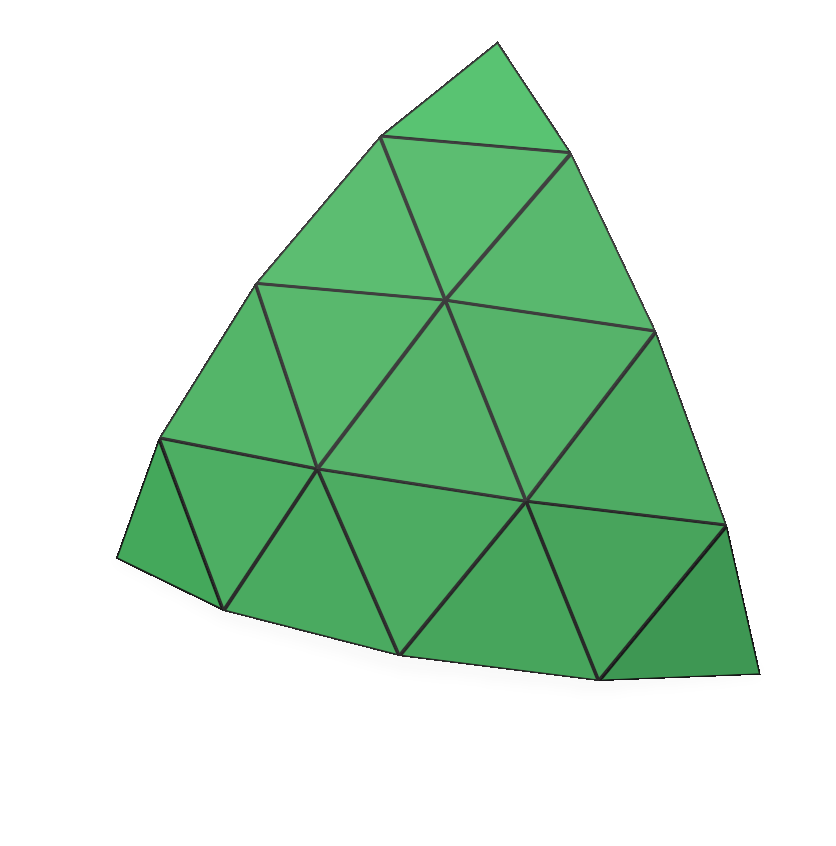
\includegraphics[width=0.3\textwidth]{figures/tessellation.png}
    \vspace{-1cm}
    \caption{Result of the tessellation}
  \end{wrapfigure}
  Note that choosing $\alpha < 1$ leads to a triangle that "curves inwards" in
  its center, while its edges still curve outwards (in pink on the figure).

  After computing the control points, it suffices to consider a tessellation of
  the triangle $\Delta$ into sub-triangles, and compute the vertices of every
  sub-triangle using $\vec{b}$. This allows for the use of a "level of details"
  parameter that can be changed if needed.

  One major advantage of curved PN triangles over some similar methods is that,
  when computing a curved PN triangle, we only need to consider one triangle.
  This allows the use of the GPU for computing curved PN triangles and their
  tessellation using, for example, a geometry shader in~\textsf{OpenGL}.

  \begin{figure}[htbp]
    \centering
    \begin{adjustbox}{center}
      \begin{tikzpicture}[box/.style={draw,rectangle,rotate=30,rounded corners,minimum height=0.4cm,text centered}, shorten >=0.3cm,shorten <=0.2cm]
        \node(a) {};
        \node[right=2.5cm of a] (b) {};
        \node[right=2.5cm of b] (c) {};
        \node[right=2.5cm of c] (d) {};
        \node[right=2.5cm of d] (e) {};
        \node[right=2.5cm of e] (f) {};
        \node[box] (va) at (a) {Vertex Specification};
        \node[box] (vb) at (b) {Vertex Shader};
        \node[box] (vc) at (c) {Geometry Shader};
        \node[box] (vd) at (d) {Primitive Assembly};
        \node[box] (ve) at (e) {Rasterization};
        \node[box] (vf) at (f) {Fragment Shader};
        \draw[very thick, ->] (va) to (vb);
        \draw[very thick, ->] (vb) to (vc);
        \draw[very thick, ->] (vc) to (vd);
        \draw[very thick, ->] (vd) to (ve);
        \draw[very thick, ->] (ve) to (vf);
      \end{tikzpicture}
    \end{adjustbox}
    \caption{\textsf{OpenGL}'s rendering pipeline (simplified)}
    \label{fig:opengl}
  \end{figure}

  A \textit{geometry shader} in \textsf{OpenGL} (figure~\ref{fig:opengl}) is a
  program that gets a triangle and transform it into some geometry (hence the
  name \textit{geometry} shader), eventually emitting multiple triangles. A
  geometry shader for producing curved PN triangles from PN triangles was
  implemented in less than 200 lines of GLSL (\linkfile{shaders/shader.geom}).

  \section{Comparing different methods for computing normals.}

  After computing the curved PN triangles and their tessellation, it is
  important to compute normals for the vertices of the new triangles, so that
  they can be passed to the fragment shader after the rasterization.

  In \cite{curvedpntriangles}, they define \textit{quadratic varying normals},
  a sort of quadratic Bézier patch (but representing normals and not
  positions). Given a triangle, they define
  \[
    \vec n(u, v, w) := \mathrm{normalized}\Big(\sum_{i+j+k = 2} \vec n_{kij} u^i v^j w^k\Big)
  ,\] 
  where Bézier control points $\vec n_{kij}$ are defined similarly to $\vec
  b_{kij}$.

  Another way of computing normals would be \textit{linear varying normals}
  (also given in~\cite{curvedpntriangles}): for a triangle whose normals are
  $\vec N_1$, $\vec N_2$ and $\vec N_3$, define \[
  \vec n(u, v, w) := \mathrm{normalized}\big( u \vec N_1 + v \vec N_2 + w \vec N_3 \big)
  .\]

  A third way of computing the normals would be "\textit{exact}" in the sense
  that it would follow exactly from the parametric surface $\vec b(u, v)$, but
  would not use directly the normals provided by the 3D model:
  \[
  \vec n (u, v, w) := \mathrm{normalized}\left(\frac{\partial \vec b(u, v, w)}{\partial u} \times \frac{\partial \vec b(u, v, w)}{\partial v} \right)
  ,\] 
  where ${-}\times {-}$ denotes the cross product. There is no need to consider
  $\partial \vec b(u, v, w) / \partial w$ as it is not independent from $u$ and
  $v$: $w = 1 - u - v$.
  Exact computations of the derivatives in terms of the Bézier control
  points~$\vec b_{kij}$ were done in Maple and results can be found in the
  shader file~\linkfile{shaders/shader.geom}.

  \begin{figure}[htbp]
    \centering
    \subcaptionbox{Linear varying normals}{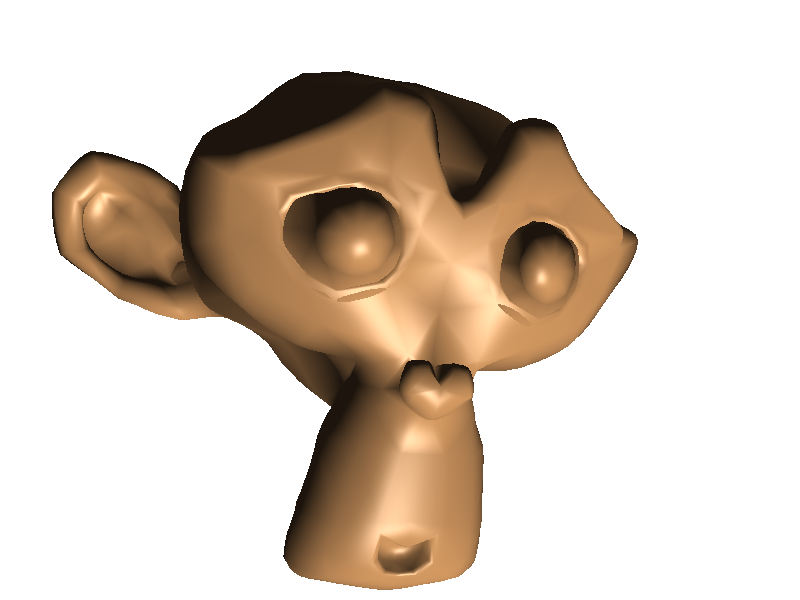
\includegraphics[width=0.32\textwidth]{figures/normals1.png}}
    \subcaptionbox{Quadratic varying normals}{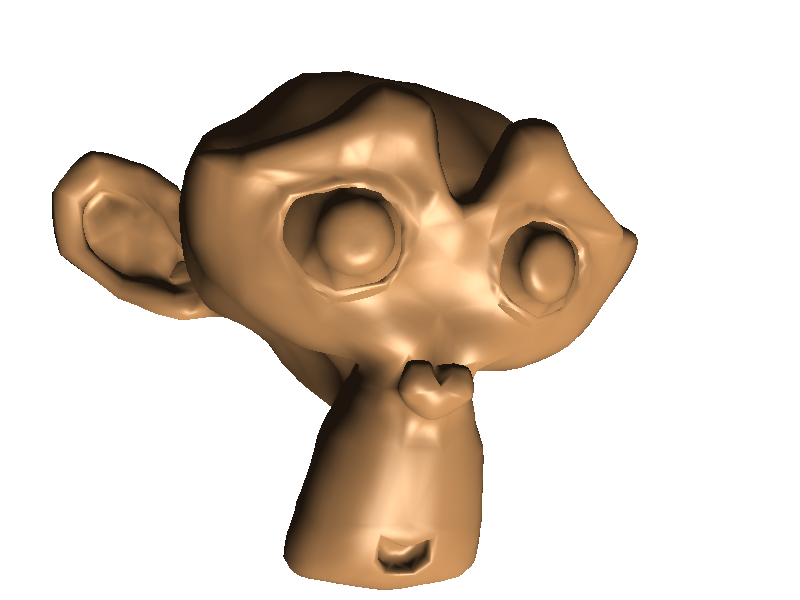
\includegraphics[width=0.32\textwidth]{figures/normals2.png}}
    \subcaptionbox{"Exact" normals}{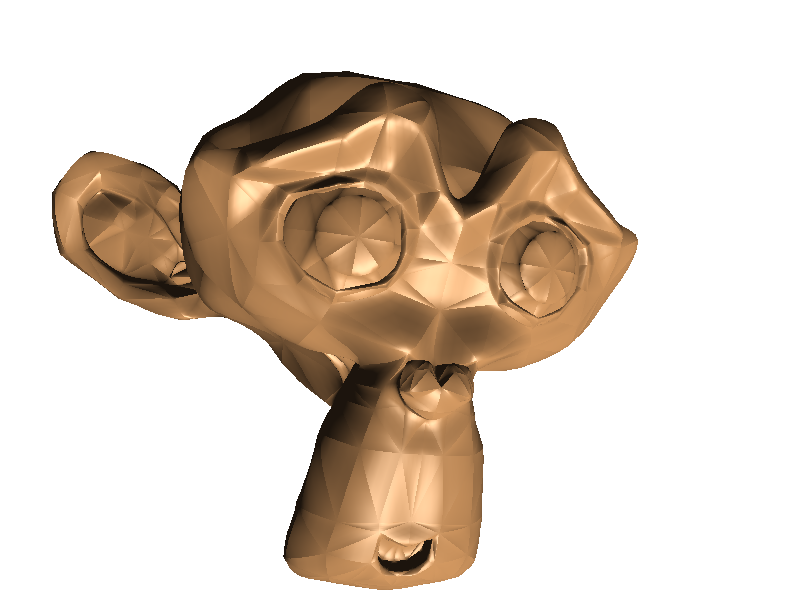
\includegraphics[width=0.32\textwidth]{figures/normals3.png}}
    \caption{Comparison of different normals-computing methods}
    \label{fig:normals}
  \end{figure}

  \begin{wrapfigure}[9]{r}{0.4\textwidth}
    \centering
    \vspace{-1cm}
    \subcaptionbox{Linear varying normals}{\vspace{-0.5cm}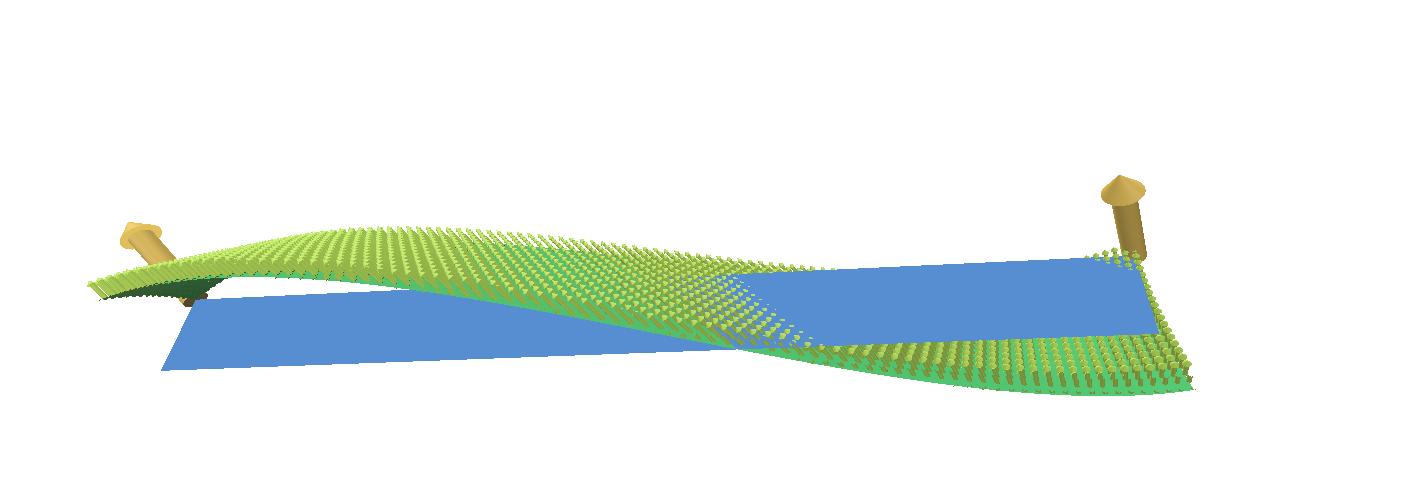
\includegraphics[width=0.37\textwidth]{figures/normals1_field.png}}
    \subcaptionbox{Quadratic varying normals}{\vspace{-0.5cm}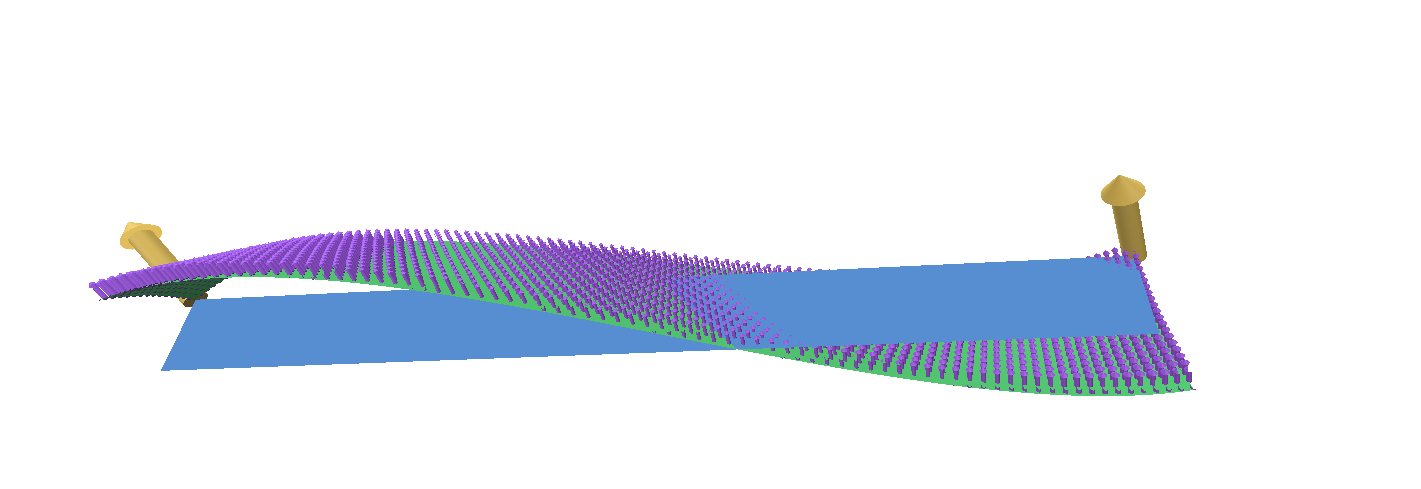
\includegraphics[width=0.37\textwidth]{figures/normals2_field.png}}
    \caption{Normals on a varying surface}
    \label{fig:normals-simplify}
  \end{wrapfigure}

  As can be seen in figure~\ref{fig:normals} (page~\pageref{fig:normals}), the
  three methods give similar results at the center of triangles. Yet, at the
  boundary, shading differs. When using Phong shading (as done in
  figure~\ref{fig:normals}, \textit{c.f.}~\linkfile{shaders/shader.frag}),
  linear varying normals seem to give better results.

  However, as stated in~\cite{curvedpntriangles}, linear varying normals can
  sometimes oversimplify the variations of the surface, as shown in
  figure~\ref{fig:normals-simplify}.

  \section{Applications of curved PN triangles.}

  \subsection{Marching cubes~\cite{marchingcubes}, procedural generation.}\label{subsect:marchingcubes}

  The \textit{marching cubes algorithm}, introduced in~\cite{marchingcubes}, allows
  us to extract an isosurface of some given function. By design, this algorithm
  produces blocky-looking results. The use of curved PN triangles would allow
  for a smoother surface without too much overhead.

  \begin{wrapfigure}[11]{l}{0.35\textwidth}
    \centering
    \vspace{-1cm}
    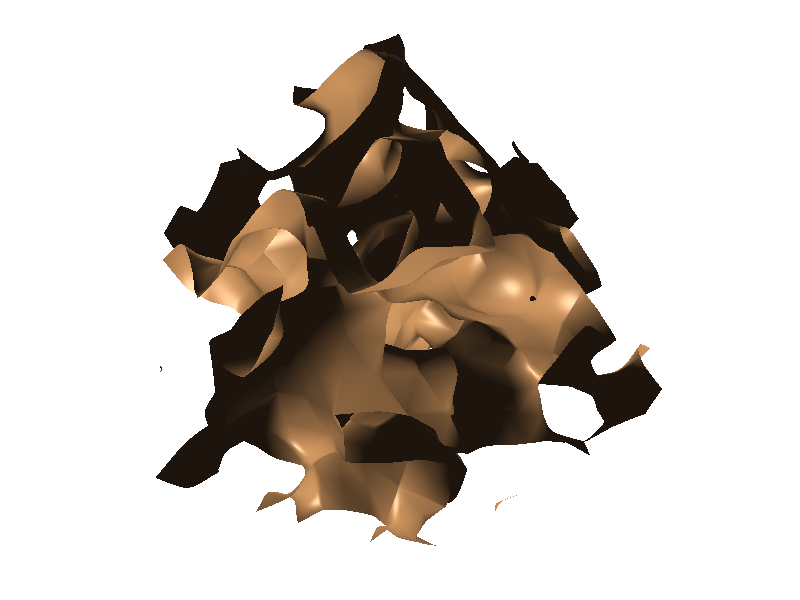
\includegraphics[width=0.45\textwidth,trim={5cm 0 0 0},clip]{figures/marching-cubes.png}
    \vspace{-1cm}
    \caption{Marching cubes on Perlin noise rendered with curved PN triangles}
  \end{wrapfigure}

  For examples, procedural cave generation can be done using the marching cube
  algorithm and some noise function like Perlin noise. In that case, no need to
  perform a lot of subdivisions on far-away parts of the cave. This can easily
  be done using curved PN triangles without having to run the marching cubes
  algorithm when a new level of details is needed. And, all the necessary data
  is already in the GPU's memory, thus no data-updates need to happen.

  A basic example of curved PN triangles applied to marching cubes on some
  Perlin noise can be found in~\linkfile{cubes.py}
  and~\linkfile{opengl\_cubes.py}.

  \subsection{Cloth simulations.}

  Consider the following cloth-simulation model: a grid in which every vertex
  is connected to its eight neighbors using springs. Thus, in this model, a
  vertex is only affected by the tension force of the springs and gravity.

  Such a simple can be easily simulated (\textit{c.f.}~\linkfile{cloth.py}),
  but this simulation can become very costly as the size of the mesh increases.
  One solution is to simulate on a coarse mesh and to use curved PN triangles
  for the rendering part (\textit{c.f.}~\linkfile{opengl\_cloth.py}). In games,
  for example, this could allow for real-time rendering without costing too
  much performance. This technique also enables the use of level of details, as
  discussed in subsection~\ref{subsect:marchingcubes}.

  \begin{figure}[htbp]
    \centering
    \subcaptionbox{Cloth mesh\label{fig:cloth-clothmesh}}{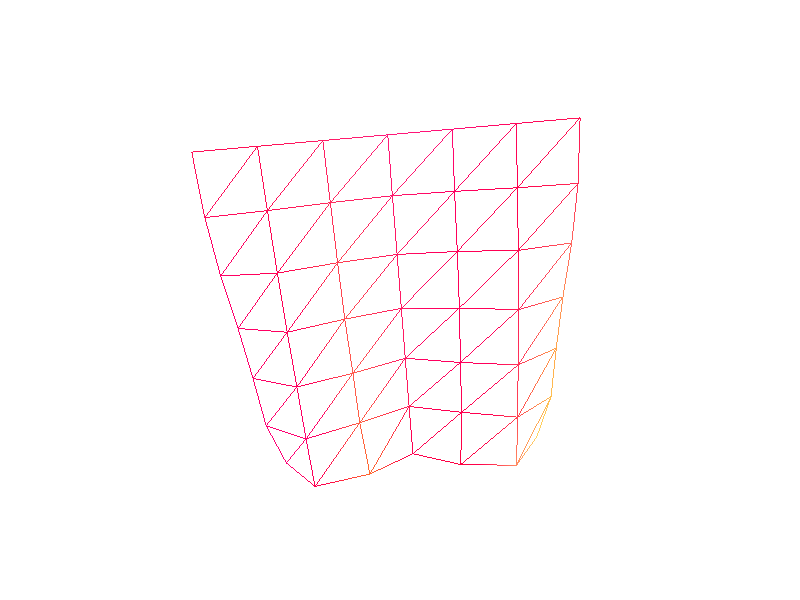
\includegraphics[trim={5cm 0 5cm 0},clip,width=0.33\textwidth]{figures/cloth-base.png}}
    \subcaptionbox{Render mesh\label{fig:cloth-rendermesh}}{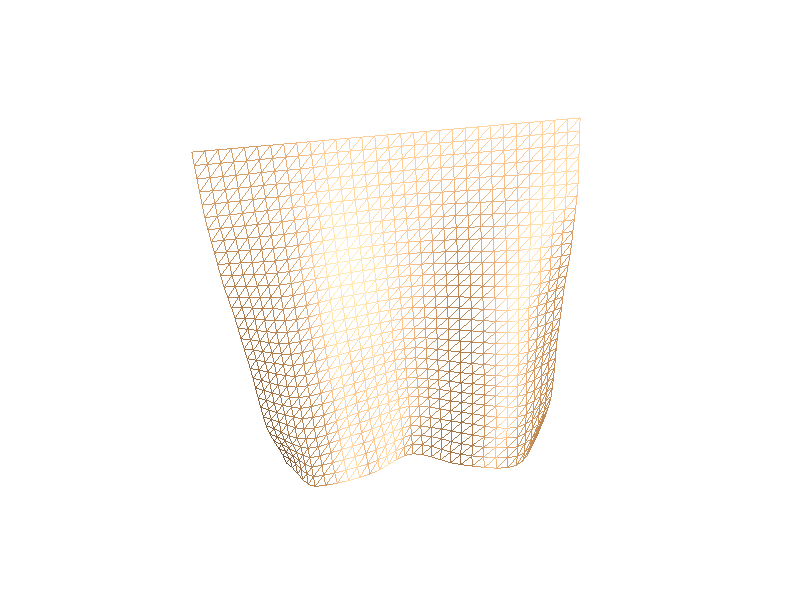
\includegraphics[trim={5cm 0 5cm 0},clip,width=0.33\textwidth]{figures/cloth-wire.png}}
    \subcaptionbox{Resulting surface}{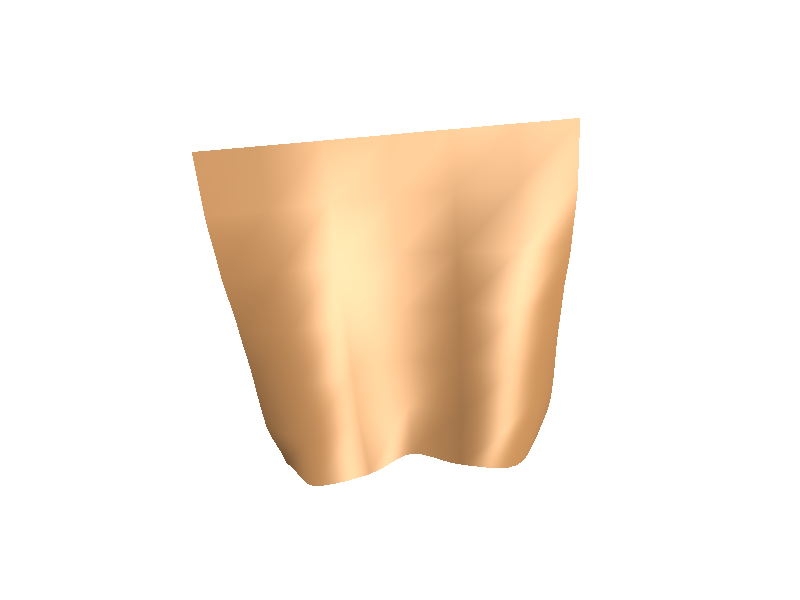
\includegraphics[trim={5cm 0 5cm 0},clip,width=0.33\textwidth]{figures/cloth-surf.png}}
    \caption{Simulation on a coarse mesh and curved PN triangles for rendering}
    \label{fig:cloth}
  \end{figure}

  Even really small grids ($7 \times 7$ in figure~\ref{fig:cloth-clothmesh})
  produce believable enough-results. Doing the simulation on the render mesh
  ($75$ times finer in the case of figure~\ref{fig:cloth-rendermesh}) would
  result in way higher computation costs (about $5\:000$ times higher with the
  details shown in figure~\ref{fig:cloth-rendermesh}). A video of the cloth
  simulation is available: \linkfile{videos/cloth-simulation.mov}.

  \section{Conclusion.}

  Curved PN triangles are a pretty inexpensive way of smoothing a mesh as it
  can be done on the GPU using, for example, a geometry shader in
  \textsf{OpenGL}. It allows the use of algorithms on some coarser meshes which
  are then rendered in a higher resolution.
  Here, only marching cubes and cloths simulations were presented, but physical
  computations, \textit{e.g.}\ finite element methods, could be done on PN
  triangles (acting on the position of vertices but also their normals) that
  are then subdivided when the strain gets too high to avoid loss of precision.
  This may not be the best option as curved PN triangles were designed for
  rendering in mind, so they may only \textit{look} smooth, whereas other
  methods like Catmull-Clark subdivision \cite{catmull} produces meshes that
  \textit{are} smooth.

  One important note is that meshes \textit{can} be designed for curved PN
  triangles-based rendering~\cite{simplification}. PLY files in the
  \linkfile{data/} folder were made using \textit{Blender} without optimizing
  the mesh for this process in mind.

  As one might suspect, curved PN triangles have some drawbacks. For example,
  even if the starting mesh is continuous, the resulting mesh can be
  discontinuous. This is usually the case when the mesh's normals are badly
  computed. Shading can also reveal the original mesh when the normals are not
  well-interpolated. Another drawback comes for the force of curved PN
  triangles: they smooth out the mesh, and thus, hard edges are also smoothed
  out. This can be fixed by changing the mesh or by updating a few terms as
  discussed in~\cite{curvedpntriangles}.

  Curved PN \textit{quads} is something that was introduced in~\cite{pnquads}
  and more work was done in~\cite{g1pnquads}. They allow for more control
  points, but the \textsf{OpenGL} pipeline does not support quads as a
  primitive.

  Code related to this project can be found on GitLab:
  \begin{center}
    \url{https://gitlab.aliens-lyon.fr/hsalou/m1-cgdi-project}.
  \end{center}

  \renewcommand\emph[1]{{\em#1}}
  \printbibliography
\end{document}
